\chapter{The Design of a Nuclear Reactor}
Following our study of cross sections and the interactions between nuclei and neutrons, we will now delve into the properties of the nuclear fuel. This chapter will explore the dependence of cross sections on energy, analyze the distributions of neutrons, and estimate the multiplication factor, \( k \).

To achieve this, we will examine how different materials within the reactor core influence reaction rates and the neutron flux distribution across the energy spectrum.


\section{Nuclear Fuel Properties}

Cross sections of fissile and fertile materials are functions of energy; therefore, many of the processes that occur inside a nuclear reactor are determined by the energy of the neutrons. The dependence on energy of the cross sections extends over a broad range from: \(10\) MeV to \(0.001\) eV. Fertile materials can undergo fission when absorbing neutrons, but only if the transfer energy surpasses a threshold. A fraction of the total neutrons will be absorbed; this fraction is also energy-dependent. This leads to the following expression:

\begin{equation}
    \eta (E) = \frac{\nu \Sigma_{f}(E)}{\Sigma_{a}(E)}
    \label{eq:first_eta_def}
\end{equation}

The expression represents the fraction of neutrons that create new neutrons after being absorbed. $\nu$ is the number of neutrons produced by fission, and $\Sigma_{x}$ represents the cross section of the fission and absorption processes. By definition, $\Sigma$ depends on the nuclei density, so we can cancel out these factors and end up with $\sigma$.

However, nuclear fuel is composed of multiple isotopes, then $\sigma_{x}$ should be adjusted to consider the mixture of isotopes. First, we have to consider the enrichment \textbf{Eq.}(\ref{eq:Atomic_enr}). We are going to label the cross sections as $\sigma_{x}^{y}$, where \(x\) indicates the process considered (\(f\) for fission and \(a\) for absorption), and \(y\) indicates the fissionable material (\(fi\) for fissile and \(fe\) for fertile). All of these considerations lead to the following expression:

\begin{flalign}
   && \eta (E) = \frac{\nu \, \Tilde{e} \, \sigma_{f}^{fi}(E) + \nu \, (1-\Tilde{e}) \, \sigma_{f}^{fe}(E)}{\Tilde{e} \, \sigma_{a}^{fi}(E) + (1-\Tilde{e}) \, \sigma_{a}^{fe}(E)} &&
    \label{eq:eta_def_fi_fe}
\end{flalign}

The changes caused by the level of enrichment are reflected on \textbf{Fig} \ref{fig:Eta_enrichment}.

\begin{figure}
    \centering
    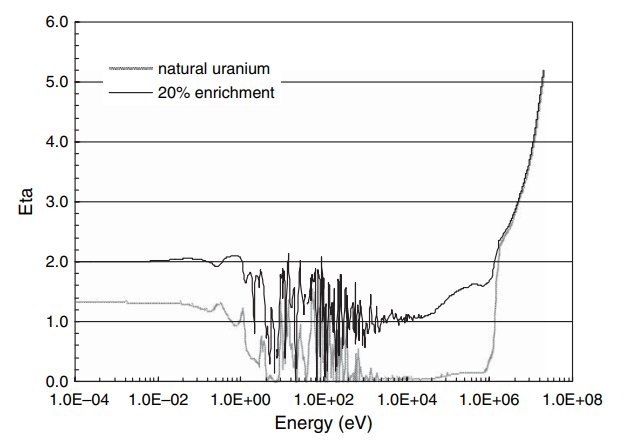
\includegraphics[width=0.75\linewidth]{Kap3/Figures_Kap3/Eta_enrichment.png}
    \caption{Figure showing two plots of $\eta$ as function of energy for uranium fuel at different levels of enrichment. From \textbf{Ref.} \cite{Lewis_2014}}
    \label{fig:Eta_enrichment}
\end{figure}

Nuclear reactors are designed to concentrate in the fast or thermal energy ranges, this is due to the valley in the intermediate energy range. As mentioned before in the document, neutrons lose energy due to elastic scattering, until they reach thermal equilibrium with the medium. There are two types of nuclear reactors, fast and thermal reactors, each one with their own specifications.

In fast reactor design inside the core any kind of material is avoided, different from fuel, so that neutrons experience few scatterings and stay in the fast energy range. Low atomic weight materials are capable to quickly reduce neutrons energy, consequently, they are avoided. This increases the possibility for uranium-238 to absorb neutrons, which depletes the amount neutrons \cite{Lewis_2014}. This makes it impossible for a fast reactor to be fueled with natural uranium \cite{Lewis_2014}; it needs of high enrichment-uranium (HEU) with $\Tilde{e} \gtrsim 10\%$. 

The opposite situation happens for thermal reactors. They need materials, called moderators, to slow-down the neutrons. A thermal nuclear reactor can operate with much lower enrichment \cite{Lewis_2014}. We must examine the properties of moderators to understand their behavior.  

\section{Slow Down Decrement}

To measure the effectiveness of a nucleus to slow neutrons down by elastic scattering, we use the slow down decrement, denoted as $\xi$. It is defined as the mean value of the logarithm of the fraction of energy lost \cite{Lewis_2014}:

\begin{flalign}
    && \xi := \overline{\ln\left(\frac{E}{E}\right)} = \int \ln\left(\frac{E}{E'}\right) p(E \rightarrow E') dE' &&
    \label{eq:def_xi}
\end{flalign}

A long deduction gives us that:
\begin{flalign}
    &&  p(E \rightarrow E') = \frac{1}{(1 - \alpha) E} dE' &&
    \label{eq:dist_energy_scatter}
\end{flalign}

Where $\alpha = \left(\frac{A-1}{A+1}\right)^{2}$, which can be replaced into \textbf{Eq.}(\ref{eq:def_xi}) resulting in:

\begin{flalign}
    && \xi = 1 + \frac{\alpha}{1 - \alpha} \ln \alpha &&
    \label{eq:def_sl_decre}
\end{flalign}

This parameter can be approximated as $\xi \approx \frac{2}{A + 2/3}$. With it, we can estimate the number of collisions necessary to reduce the energy of a neutron from fast neutrons to thermal neutrons. For instance, consider \(E_{1}, E_{2}, \dots, E_{n}\) to be the neutron energies after the \(i\)-th collision, this would be:

\begin{flalign}
    && \ln\left(\frac{E_{0}}{E_{n}}\right) = \ln\left(\frac{E_{0}}{E_{1}}\right) + \ln\left(\frac{E_{1}}{E_{2}}\right) + \dots + \ln\left(\frac{E_{n-1}}{E_{n}}\right) &&
\end{flalign}

Replacing each of the terms for the average logarithmic energy loss \(\xi\), we have:

\begin{flalign}
   && n = \frac{1}{\xi} \ln\left(\frac{E_{0}}{E_{n}}\right) &&
\end{flalign}

Evaluating the expression for hydrogen, we get $n \approx 18$. However, this expression considers only one kind of nucleus. In order to consider the effects of other isotopes, we have to make an average over their \(\xi\), resulting in:

\begin{flalign}
    && \overline{\xi} = \frac{1}{\Sigma_{s}} \sum_{i} \xi_{i} \Sigma_{si} &&
    \label{eq:def_ave_sd_decre}
\end{flalign}

The concept of the slow down decrement is crucial in understanding how neutrons lose energy through collisions. This directly impacts the design and efficiency of neutron moderators, which are essential components in thermal reactors.

\section{Neutron Moderators}

Thermal reactors must reduce the neutrons' energy with as few collisions as possible so that they make the transit to the thermal region without being absorbed in resonance processes \cite{Lewis_2014}. The slowing down decrement is the parameter most suitable for this purpose.

A good moderator must possess additional properties, beyond just a high slowing down decrement. One crucial property is the slowing down power, defined as $\xi \Sigma_s$, where $\Sigma_s$ is the macroscopic scattering cross section. This parameter indicates the effectiveness of a material in slowing down neutrons through scattering interactions. A high slowing down power ensures that neutrons lose energy efficiently during collisions.

Another important parameter is the slowing down ratio, which is the ratio of the material's slowing down power to its thermal absorption cross section, $\Sigma_a (\text{thermal})$. This ratio indicates how well a material can slow down neutrons without absorbing them. A high slowing down ratio is desirable because it means the material can effectively moderate neutrons to thermal energies while minimizing neutron absorption.

For example, heavy water (D$_2$O) has a high slowing down ratio, making it an excellent moderator for reactors using natural uranium fuel. On the other hand, materials with lower slowing down ratios, such as ordinary water (H$_2$O), require enriched uranium fuel to achieve efficient moderation.

\begin{table}[h]
    \caption{Slowing Down Properties of Common Moderators. From \textbf{Ref.} \cite{Lewis_2014}}
        \begin{tabular}{lccc}
            \toprule
            & Slowing Down Decrement  & Slowing Down Power  & Slowing Down Ratio \\
            \multirow{1}{*}{Moderator}
            & $\xi$ & $\xi\Sigma_s$ & $\frac{\xi\Sigma_s}{\Sigma_a (\text{thermal})}$ \\
            \midrule
            H$_2$O & 0.93 & 1.28 & 58 \\
            D$_2$O & 0.51 & 0.18 & 21,000 \\
            C      & 0.158 & 0.056 & 200 \\
            \bottomrule
        \end{tabular}
\end{table}

\subsection{Energy Spectra of Neutrons}

Having discussed moderation, it is time to study the energy spectra of neutrons. This energy spectrum results from the competition between scattering and absorption reactions.

Neutrons with kinetic energies around the thermal range lose energy during scattering processes. In contrast, thermal neutrons do not lose energy because they are in thermal equilibrium with the medium. When the reactor medium has both, a large average energy loss per collision and a high ratio of scattering to absorption cross-sections, neutrons follow a distribution close to thermal equilibrium, known as soft, or thermal, spectrum. Conversely, systems that do not meet these conditions are characterized by a distribution close to the fission spectrum, known as hard, or fast, spectrum.

We can express this distribution in terms of the density distribution $\Tilde{n}'''(E)dE$, which is the number of $\text{neutrons}/\text{cm}^{3}$ with energies between $E$ and $E + dE$. However, the neutron flux frequently, defined as:

\begin{equation}
    \varphi(E) = v(E)\Tilde{n}'''(E)
    \label{eq:neutron_flux}
\end{equation}

where \(v(E)\) corresponds to the speed of a neutron with kinetic energy \(E\). Together with the macroscopic cross-section \textbf{Eq.}(\ref{eq:def_macs}), we can construct the probability distribution of the number of collisions of type \(x\), per \(\text{cm}^{3}\) per second, for neutrons with energy between $E$ and $E + dE$ as:

\begin{equation}
    \Sigma_{x}(E)\varphi(E)dE
\end{equation}

Integrating over all energy, we get the probable number of collisions of type \(x\) per \(\text{cm}^{3}\) per second for all neutrons \cite{Lewis_2014}.

For instance, consider the scenario where a collision removes a neutron, either by absorption or scattering, from the energy region \(E\) and \(E + dE\). However, neutrons colliding from another energy region, say \(E'\) and \(E' + dE'\), enter the first region. When the number of neutrons leaving the region and entering it are equal, we have a stationary state \cite{Lewis_2014}.

An expression for the balance situation can be deduced by using $\Sigma_{t}(E) = \Sigma_{s}(E) + \Sigma_{a}(E)$ and the probability that a neutron scattered from the energy region \(E' + dE'\) ends up in \(E + dE\), denoted as \(P(E' \rightarrow E)\) and \(P(E \rightarrow E')\). Additionally, we have to consider the prompt neutrons, whose number will be \(\chi(E)\) \textbf{Eq.}(\ref{eq:dist_fission_neutrons}) multiplied by the number of neutrons produced in each fission, denoted as \(s_{f}'''\). This results in:

\begin{flalign}
    && \Sigma_{t}(E)\varphi(E) = \int P(E' \rightarrow E) \Sigma_{s}(E')\varphi(E')dE' + \chi(E)s_{f}''' &&
    \label{eq:balanced_equation}
\end{flalign}

We already know the distribution of \(P(E' \rightarrow E)\) from \textbf{Eq.}(\ref{eq:dist_energy_scatter}). The \textbf{Eq.}(\ref{eq:balanced_equation}) is known as the balanced equation. Finally, we can define the parameter \(\Sigma_{s}(E' \rightarrow E) = p(E' \rightarrow E)\Sigma_{s}(E')\) for brevity. Now we are going to delve into the three different regions introduced before and, using the balanced equation, deduce the flux.

\subsection{Fast Neutrons}

This energy range is dominated by fission neutrons that have suffered almost no collisions because even one collision can dissipate too much energy. Using this idea, we can approximate the distribution as:

\begin{equation}
    \varphi(E) \approx \frac{\chi(E)S_{f}'''}{\Sigma_{t}(E)}
\end{equation}

This distribution is deformed by inelastic interactions and absorption processes. In fast reactors, neutrons are absorbed before they experience many collisions and reach the low-energy tail of the distribution.

\subsection{Intermediate Neutrons}

Having talk about the upper energy range in the distribution of neutrons, we must explored the range where the thermal motion of nuclei must be considered in our calculation. 

Before we delve into this distribution we have to introduce the concept of slowing-down density denoted as \(q(E)\) \cite{Lewis_2014}. 

\subsubsection{Slowing Down Density}
The slowing-down density, \(q(E)\), is defined as the number of neutrons slowing down below energy \(E\) per \(cm^{3}\) per second \cite{Lewis_2014}.

For energies around \(1.0 \, \text{eV}\), neutrons can gain energy through collisions with the medium \cite{Notas_sanabricas}. Every fission neutron produced over the energy range \(1.0 \, \text{eV} - 0.1 \, \text{MeV}\) will arrive to this range if it is not absorbed. This fact can be expressed as:

We can express the source term \(q(E)\) as follows:

\begin{flalign}
    && q(E) = \underbrace{\int_{E}^{\infty} \chi(E')s_{f}'''dE'}_{\text{Term 1}} - \underbrace{\int_{E}^{\infty} \Sigma_{a}(E')\varphi(E')dE'}_{\text{Term 2}} &&
    \label{eq:def_sdd}
\end{flalign}

Here, term 1 represents the contribution from the fission, which produce neutron with energy greater than energy \(E\), and term 2 represents the neutrons absorbed before arriving to energies below \(E\). We can make the following approximation: \(\chi(E) \approx 0\) for \(E <0.1 \, \text{MeV}\), then the integral $\int_{E}^{\infty} \chi(E')dE' \approx \int_{0}^{\infty} \chi(E')dE' = 1$ is justified. This leads to the approximation of \(q(E)\):

\begin{flalign*}
    && q(E) \approx s_{f}''' - \int_{E}^{\infty} \Sigma_{a}(E')\varphi(E')dE'&&
\end{flalign*}

By taking the derivative of the expression, we end up with $\frac{d}{dE}q(E) = - \Sigma_{a}(E)\varphi(E)$. This means that an increase in $\Sigma_{a}(E)$ causes a decrease in the slowing-down density. In the intermediate region, most of the contribution to absorption comes from resonances. Additionally, cross section between resonances are small enough to be ignored \cite{Lewis_2014}. Finally, if we are below the energy range where fission neutrons are produced, then we can simplify \textbf{Eq.}(\ref{eq:balanced_equation}) to :

\begin{flalign}
    && \Sigma_{s}(E)\varphi(E) = \int_{E}^{E/\alpha} p(E' \rightarrow E)\Sigma_{s}(E')\varphi(E')dE' &&
    \label{eq:relation_phi}
\end{flalign}

By solving the integral equation, we can establish the relation $\Sigma_{s}(E)\varphi(E) = \frac{C}{E}$. Since we are interested in the neutrons that will scattered in the interval \(\alpha\, E'' \leq E\), we will consider only with initial energy between \(E < E' < E/\alpha \). Considering this we can end up with the following expression for \(q\):

\begin{flalign*}
    && q = \int_{E}^{E/\alpha} \left[ \int_{\alpha\,E'}^{E}\frac{1}{(1-\alpha)E'} \frac{C}{E}dE''\right] dE' &&
\end{flalign*}

Solving the integral, we end up with:

\begin{flalign*}
    && q(E) = \underbrace{\left[ 1 + \frac{\alpha}{1-\alpha} \ln \alpha\right]}_{\text{Term 1}} C &&
\end{flalign*}

The similarity of the first term 1 to \(\xi\) in \textbf{Eq.}(\ref{eq:def_sl_decre}) is noticeable. Using this result and the solution for \textbf{Eq.}(\ref{eq:relation_phi}) we get and expression for \(\varphi\):

\begin{flalign}
    && \varphi(E) \approx \frac{q(E)}{\xi\,\Sigma_{s}(E)E} &&
    \label{eq:flux_interm}
\end{flalign}

Once again, we can improve this expression to consider multiple isotopes and materials by using \textbf{Eq.}(\ref{eq:def_ave_sd_decre}).

\subsection{Thermal Neutrons}
After some time and several collisions, the energy of neutrons will drop below \(0.1 \, \text{eV}\). At this point, further collisions may either absorb or release energy. Subsequently, neutrons reach thermal equilibrium with the medium at, say, temperature T, which is the one of the reactor. In this region of energy, the term related to fission neutrons in \textbf{Eq.}(\ref{eq:balanced_equation}) vanishes \cite{Lewis_2014}. A first approximation is to consider that the neutron flux follows Maxwell-Boltzmann distribution:

\begin{flalign}
    && \varphi(E) \approx \varphi_{MB}(E) = \frac{1}{(kT)^2} \exp(-E/(kT)) &&
\end{flalign}

However, the scenario is not that simple, as many neutrons are absorbed before reaching thermal equilibrium. Consequently, thermal neutrons do not follow a Maxwell-Boltzmann distribution, as their distribution is shifted towards higher energies. Describing these circumstances is not an easy task, since neutrons collide with atoms or even with the lattice of the material, complicating the calculations \cite{Notas_sanabricas}.

An approximation is to use a Maxwell-Boltzmann distribution but with an effective temperature \(T_{k} > T\):

\begin{align}
    \varphi(E) \approx \varphi_{MB}(E; T_{k}) \nonumber \\
    T_{k} = T + a\left(\frac{\Sigma_{a}}{\xi \Sigma_{s}}\right)
\end{align}

Where \(a\) is a fitted constant.

\section{Reaction Rates Averaged Over Energy}

The ability to sustain a chain reaction greatly depends on the distribution of neutrons across the energy range, which in turn depends on the composition of the different materials in the core and their effectiveness in slowing down neutrons \cite{Lewis_2014}. For this reason, cross sections must be averaged over the entire energy spectrum. We define the average cross section as:

\begin{flalign}
    && \Bar{\Sigma}_{x} = \left. \int_{0}^{\infty} \Sigma_{x}(E) \varphi(E) \, dE \right/ \int_{0}^{\infty} \varphi(E) \, dE &&
\end{flalign}

\vspace{1em}

From the definition of \(\Sigma_{x}\) in \textbf{Eq.}(\ref{eq:def_macs}), it is possible to use \(\sigma\) by canceling the atom density. The flux can be expressed as the product of the mean speed and the density of neutrons:

\begin{equation}
    \phi = \Bar{v} n'''
\end{equation}

From this relation, the mean velocity can be defined as:

\begin{flalign}
    && \Bar{v} = \left. \int_{0}^{\infty} v(E) \Tilde{n}'''(E) \, dE \right/ \int_{0}^{\infty} \Tilde{n}'''(E) \, dE &&
\end{flalign}

A more precise treatment of neutron populations requires cross section averaging over specific energy ranges rather than the entire energy spectrum \cite{Lewis_2014}. The reaction rates should be partitioned as:

\begin{flalign}
    \int \sigma_{x}(E) \varphi(E) \, dE = \int_{T} \sigma_{x}(E) \varphi(E) \, dE + \int_{I} \sigma_{x}(E) \varphi(E) \, dE + \int_{F} \sigma_{x}(E) \varphi(E) \, dE &&
    \label{eq:def_avg_cross_over_energy}
\end{flalign}

\vspace{1em}

Here, T denotes the thermal region (\(0 \leq E \leq 1.0 \, \text{eV}\)), I denotes the intermediate or resonance region (\(1.0 \, \text{eV} \leq E \leq 0.1 \, \text{MeV}\)), and F denotes the fast region (\(0.1 \, \text{MeV} \leq E \leq \infty\)). This can be written as the sum of each averaged energy:

\begin{equation*}
    \Bar{\sigma}_{x} \phi = \Bar{\sigma}_{xT} \phi_{T} + \Bar{\sigma}_{xI} \phi_{I} + \Bar{\sigma}_{xF} \phi_{F}
\end{equation*}

\vspace{1em}

This expression is obtained by multiplying and dividing \textbf{Eq.}(\ref{eq:def_avg_cross_over_energy}) by:

\begin{flalign*}
    && \phi_{\Omega} = \int_{\Omega} \varphi(E) \, dE, \quad \Omega = \text{T, I, F} &&
\end{flalign*}

Defining the energy-averaged cross section as:

\begin{flalign}
    &&\Bar{\sigma}_{x\Omega} = \left. \int_{\Omega} \sigma_{x}(E) \varphi(E) \, dE \right/ \int_{\Omega} \varphi(E) \, dE, \quad \Omega = \text{T, I, F} &&
\end{flalign}

More advanced approximations, known as multi-group methods, divide the spectrum into more than three intervals.


\section{Multiplicative Factor for Infinite Media}
This discussion introduces the concept of the infinite multiplication factor \(k_{\infty}\), which is defined by the multiplication factor \textbf{Eq.}(\ref{eq:def_multiplicative_factor}) for a reactor with an infinite medium approximation. The term ``infinite'' refers to the assumption of an unbounded medium, and it is also assumed that all neutrons are generated instantaneously.

To account for the finite volume of the reactor, we introduce the non-leakage probability:

\begin{equation}
    k = k_{\infty} P_{NL}
    \label{eq:infinite_multiplicative_factor}
\end{equation}

Here, \(P_{NL}\) is the probability that a neutron does not leak from the reactor before being absorbed. This factor depends on the geometry, the volume of the core, the distribution, and the composition of the materials within the reactor \cite{Lewis_2014}. 

An expression for \(k_{\infty}\), derived from the definition and using energy-averaged cross sections and flux given in the previous section, is:

\begin{equation}
    k_{\infty} = \left. \nu \Bar{\Sigma}_{f} \right/ \Bar{\Sigma}_{a}
    \label{eq:def_infty_sigmas}
\end{equation}

It is crucial to note that only fissionable materials contribute to \(\Bar{\Sigma}_{f}\), while \(\Bar{\Sigma}_{a}\) considers all the materials composing the reactor core \cite{Lewis_2014}.

In the next chapter, we will delve deeper into the study of this parameter and ultimately determine the equations that describe the behavior of a reactor.